In this section, we show both \textbf{query trees} and \textbf{MySQL execution plan} for the first \emph{non-optimized} and \emph{final optimized} version of each query. Moreover, we provide \emph{parallel query processing reports} for each query. This illustrates the optimization of the query statements that might include \emph{schema, query rewriting, semantic and statistical heuristics}.

\subsection{Query 1}

\subsubsection{Execution Plan Before Optimization}
\begin{figure}[H]
    \centering
    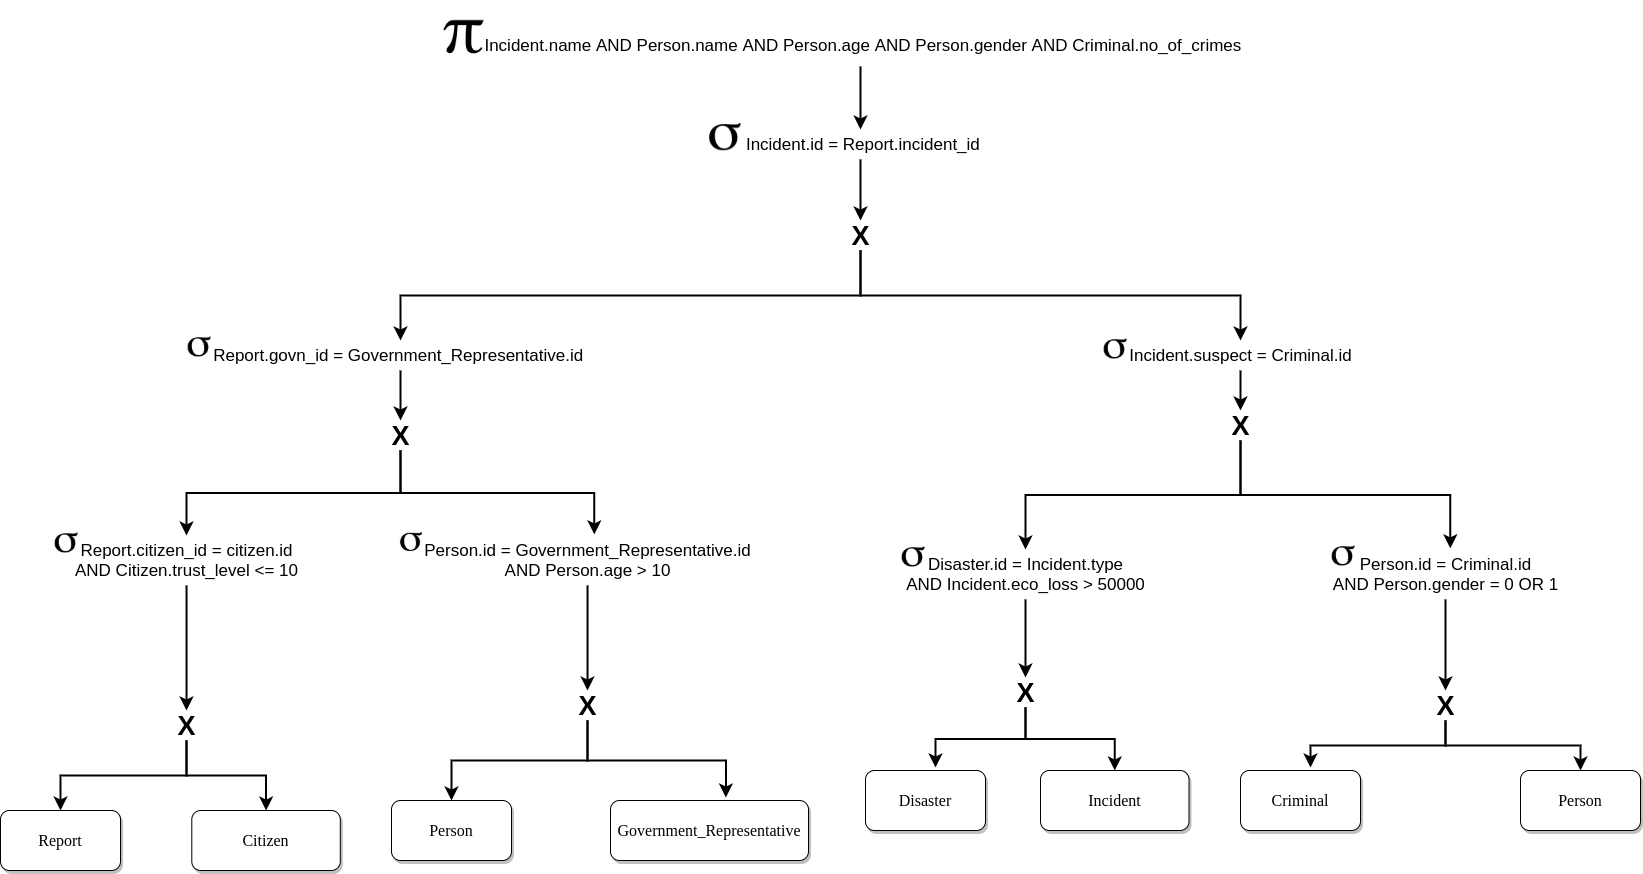
\includegraphics[width=0.8\textwidth]{images/query_trees/query1-non-optimized.png}
    \caption{Query tree for non-optimized query 1}
\end{figure}
\begin{figure}[H]
    \centering
    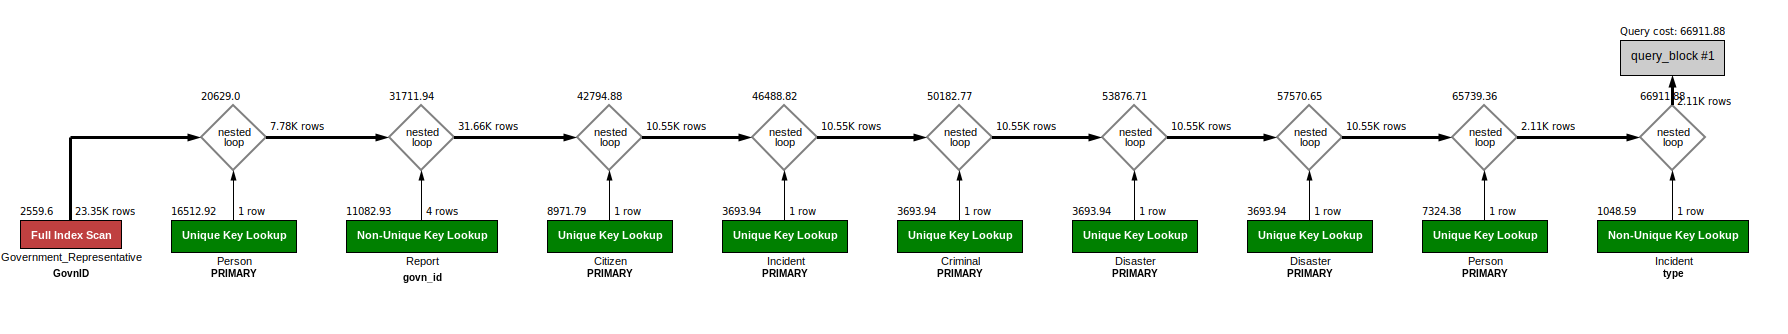
\includegraphics[width=\textwidth]{images/execution_plans/q1-1-old.png}
    \caption{Visual execution plan for non-optimized query 1}
\end{figure}

\subsubsection{Execution Plan After Optimization}
\begin{figure}[H]
    \centering
    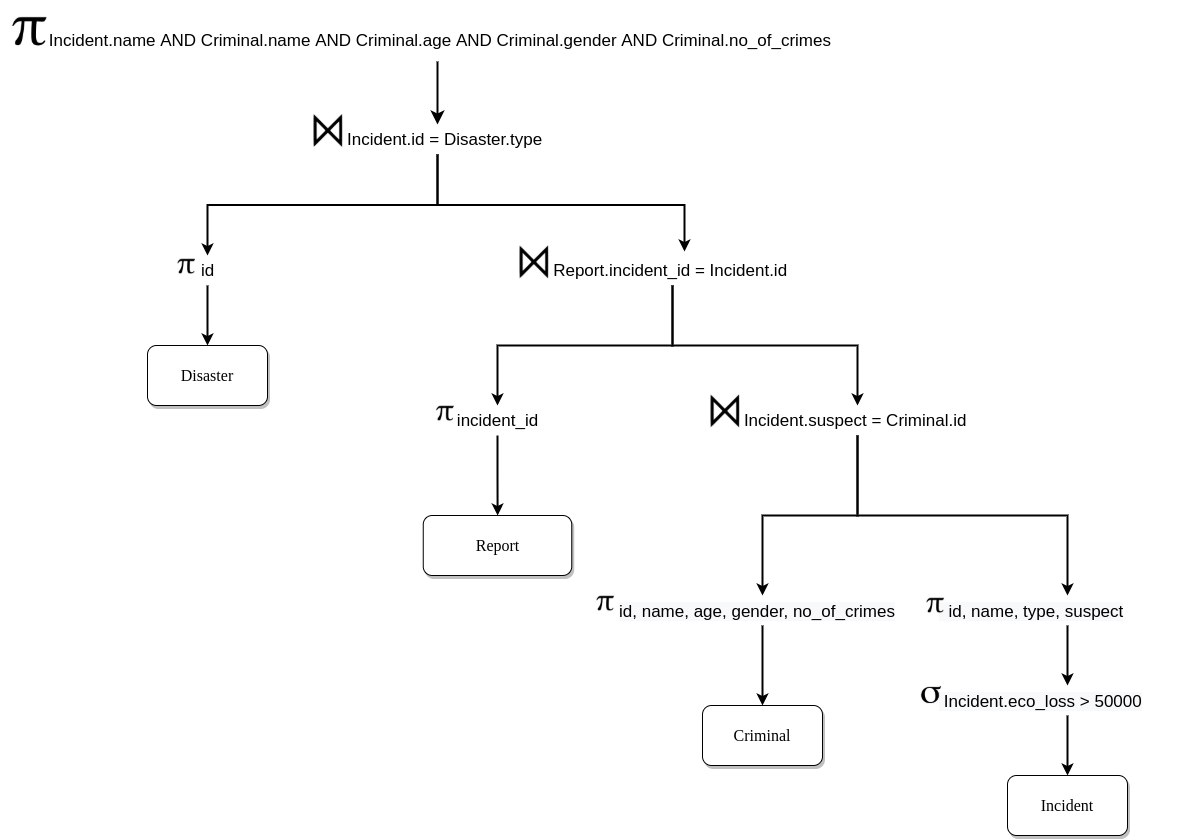
\includegraphics[width=0.8\textwidth]{images/query_trees/query1-optimized.png}
    \caption{Query tree for optimized query 1}
\end{figure}
\begin{figure}[H]
    \centering
    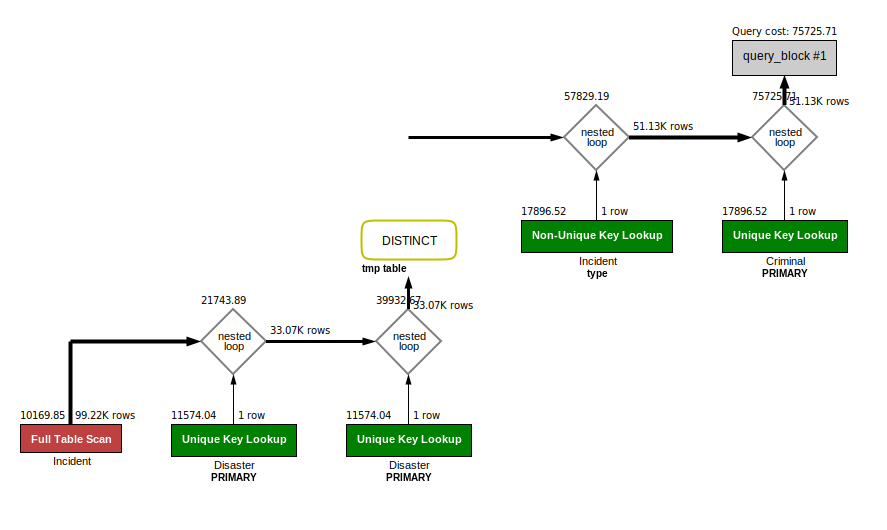
\includegraphics[width=\textwidth]{images/execution_plans/q1-3-new.png}
    \caption{Visual execution plan for optimized query 1}
\end{figure}

\subsection{Query 2}

\subsubsection{Execution Plan Before Optimization}
\textbf{Note that,} due to the huge execution time of the query before adding the indexes, we can't extract the actual non-optimized visual execution plan. Therefore, we included the visual execution plan after \emph{index optimization}. 
% \begin{figure}[H]
%     \centering
%     \includegraphics[width=0.8\textwidth]{images/query_trees/query2-non-optimized.png}
%     \caption{Query tree for non-optimized query 2}
% \end{figure}
\begin{figure}[H]
    \centering
    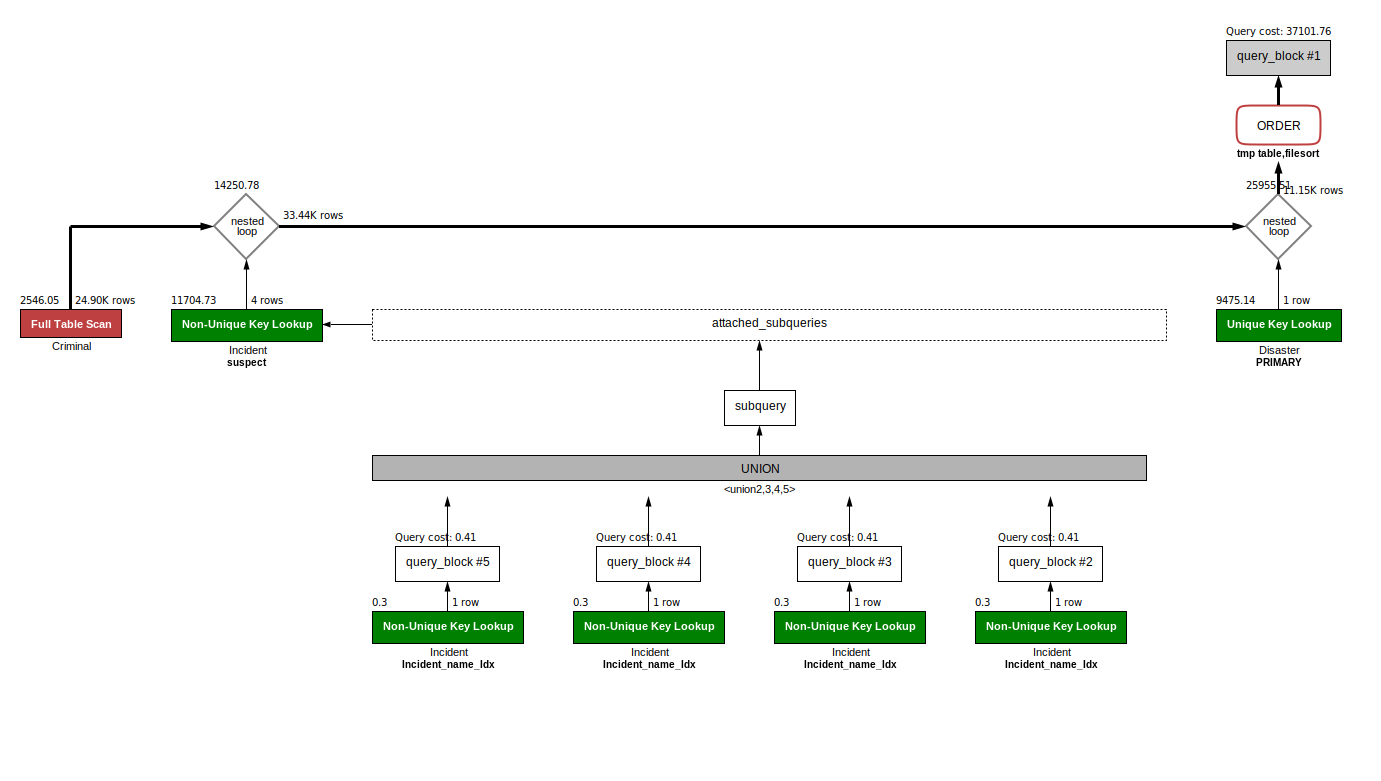
\includegraphics[width=\textwidth]{images/execution_plans/q2-2-new.png}
    \caption{Visual execution plan for non-optimized query 2}
\end{figure}

\subsubsection{Execution Plan After Optimization}
% \begin{figure}[H]
%     \centering
%     \includegraphics[width=0.8\textwidth]{images/query_trees/query2-optimized.png}
%     \caption{Query tree for optimized query 2}
% \end{figure}
\begin{figure}[H]
    \centering
    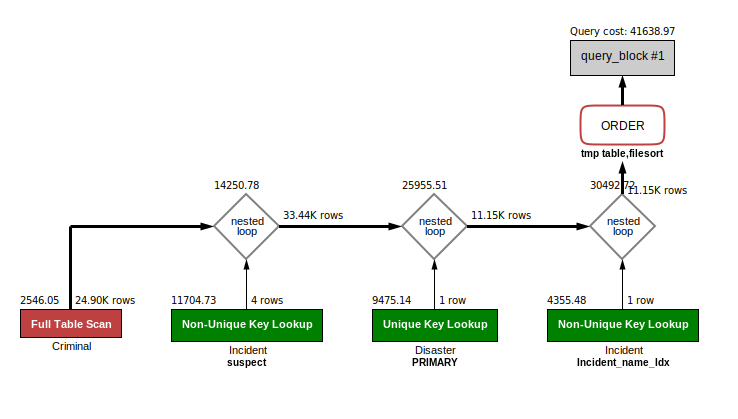
\includegraphics[width=\textwidth]{images/execution_plans/q2-4-new.png}
    \caption{Visual execution plan for optimized query 2}
\end{figure}

\subsection{Query 3}

\subsubsection{Execution Plan Before Optimization}
\begin{figure}[H]
    \centering
    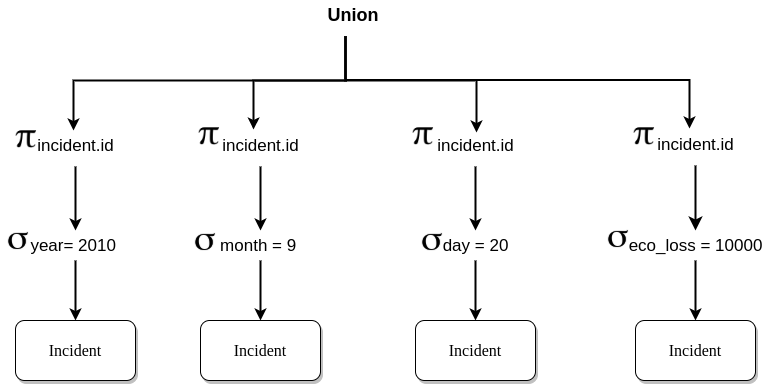
\includegraphics[width=0.5\textwidth]{images/query_trees/query3-optimized-and-non-optimized.png}
    \caption{Query tree for non-optimized query 3}
\end{figure}
\begin{figure}[H]
    \centering
    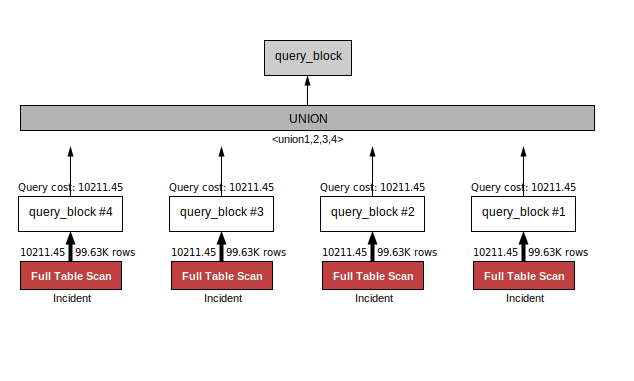
\includegraphics[width=\textwidth]{images/execution_plans/q3-1-old.png}
    \caption{Visual execution plan for non-optimized query 3}
\end{figure}

\subsubsection{Execution Plan After Optimization}
\begin{figure}[H]
    \centering
    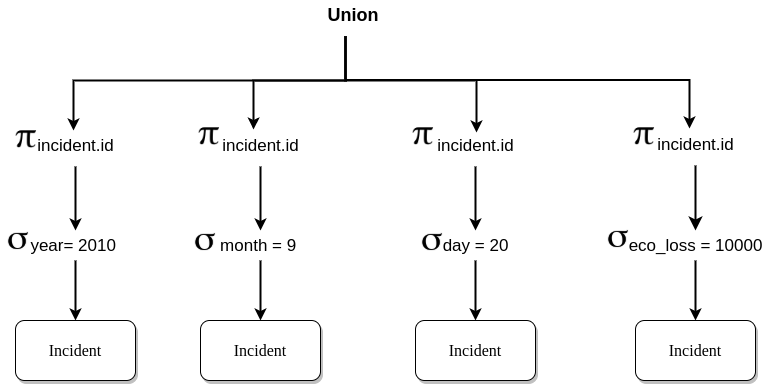
\includegraphics[width=0.5\textwidth]{images/query_trees/query3-optimized-and-non-optimized.png}
    \caption{Query tree for optimized query 3}
\end{figure}
\begin{figure}[H]
    \centering
    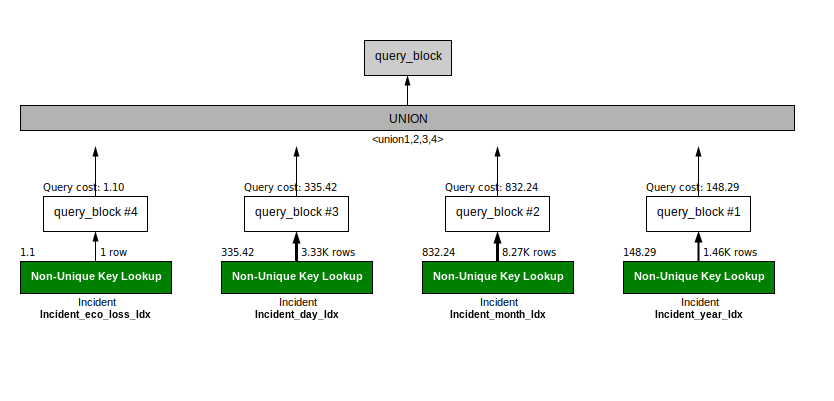
\includegraphics[width=\textwidth]{images/execution_plans/q3-3-new.png}
    \caption{Visual execution plan for optimized query 3}
\end{figure}

\subsection{Query 4}

\subsubsection{Execution Plan Before Optimization}
\begin{figure}[H]
    \centering
    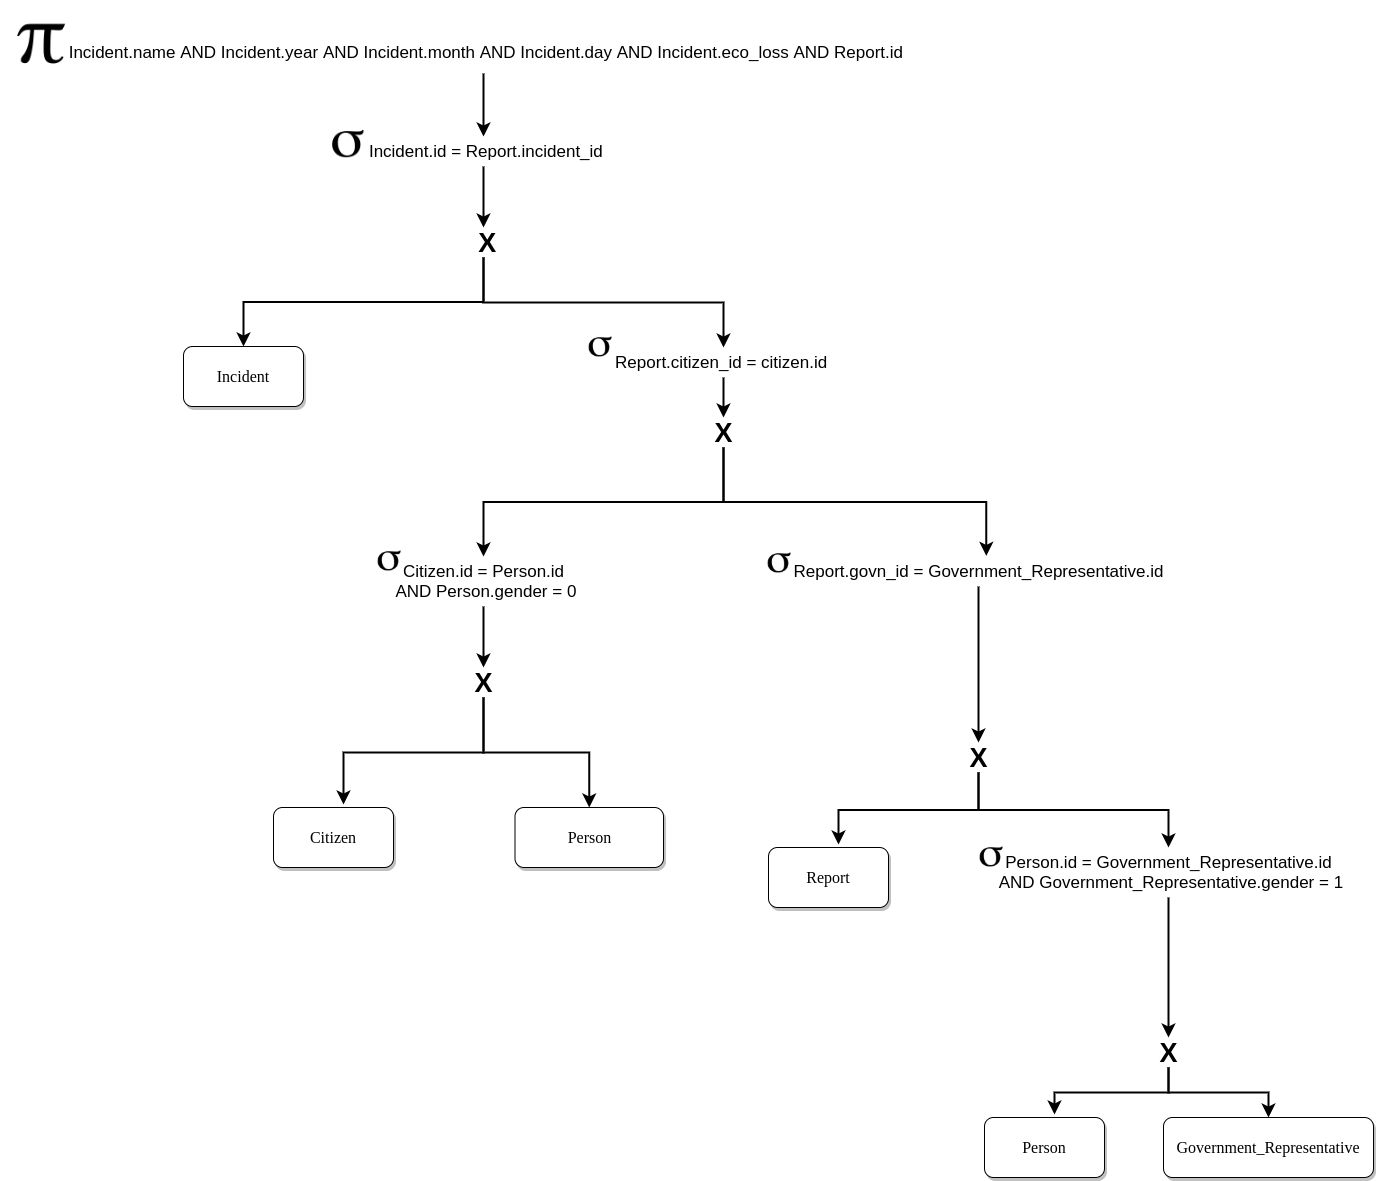
\includegraphics[width=0.8\textwidth]{images/query_trees/query4-non-optimized.png}
    \caption{Query tree for non-optimized query 4}
\end{figure}
\begin{figure}[H]
    \centering
    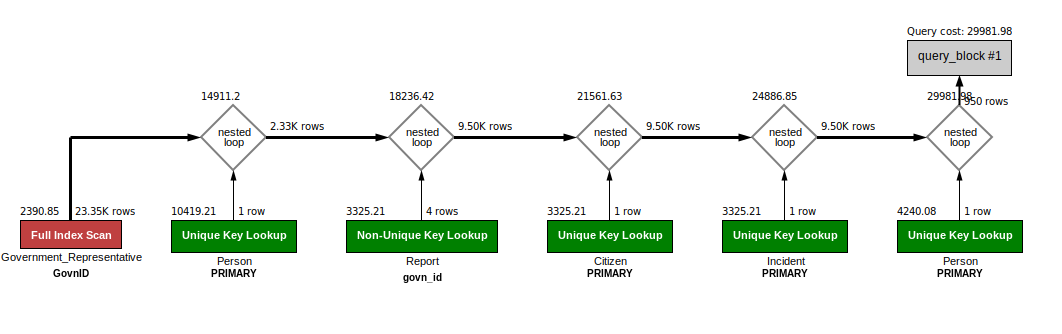
\includegraphics[width=\textwidth]{images/execution_plans/q4-1-old.png}
    \caption{Visual execution plan for non-optimized query 4}
\end{figure}

\subsubsection{Execution Plan After Optimization}
\begin{figure}[H]
    \centering
    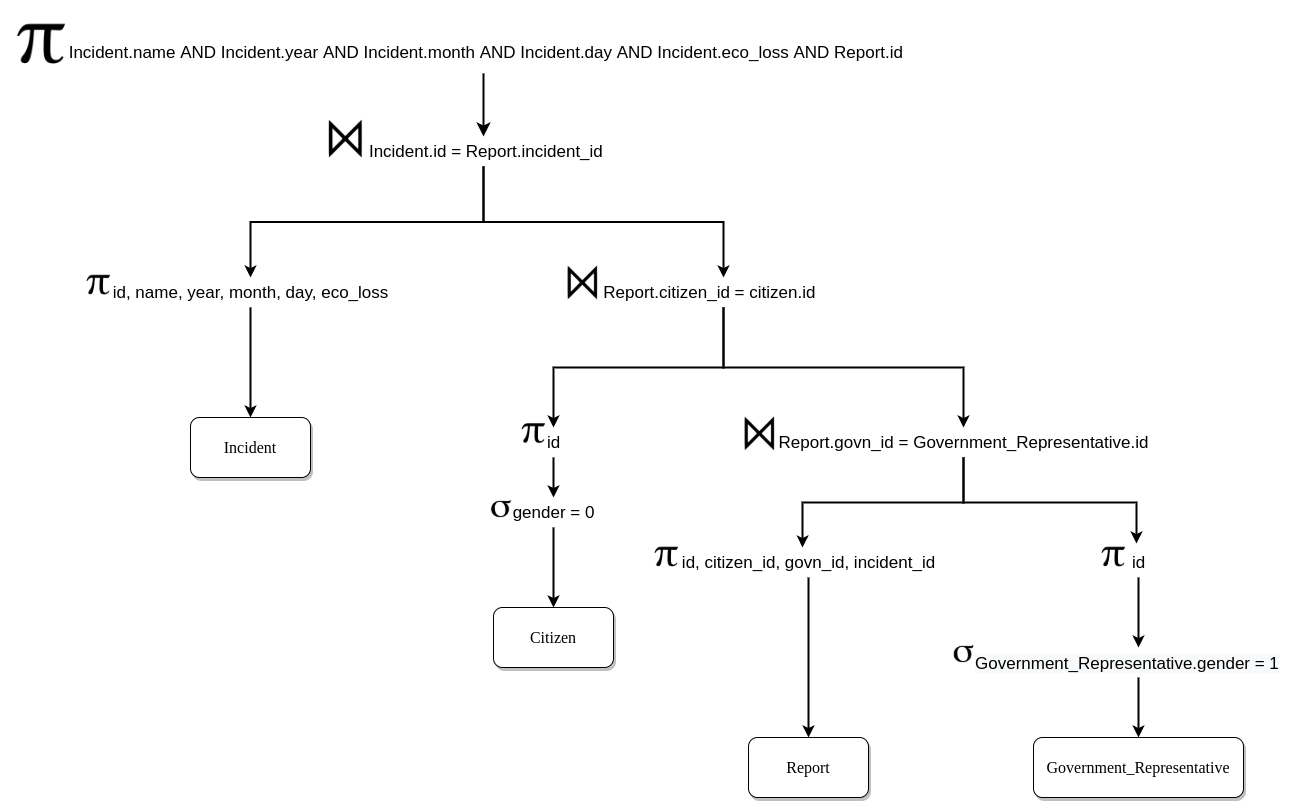
\includegraphics[width=0.8\textwidth]{images/query_trees/query4-optimized.png}
    \caption{Query tree for optimized query 4}
\end{figure}
\begin{figure}[H]
    \centering
    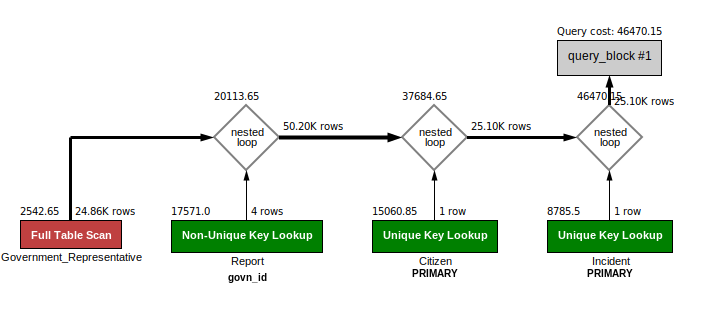
\includegraphics[width=\textwidth]{images/execution_plans/q4-2-new.png}
    \caption{Visual execution plan for optimized query 4}
\end{figure}

\subsection{Query 5}

\subsubsection{Execution Plan Before Optimization}
\begin{figure}[H]
    \centering
    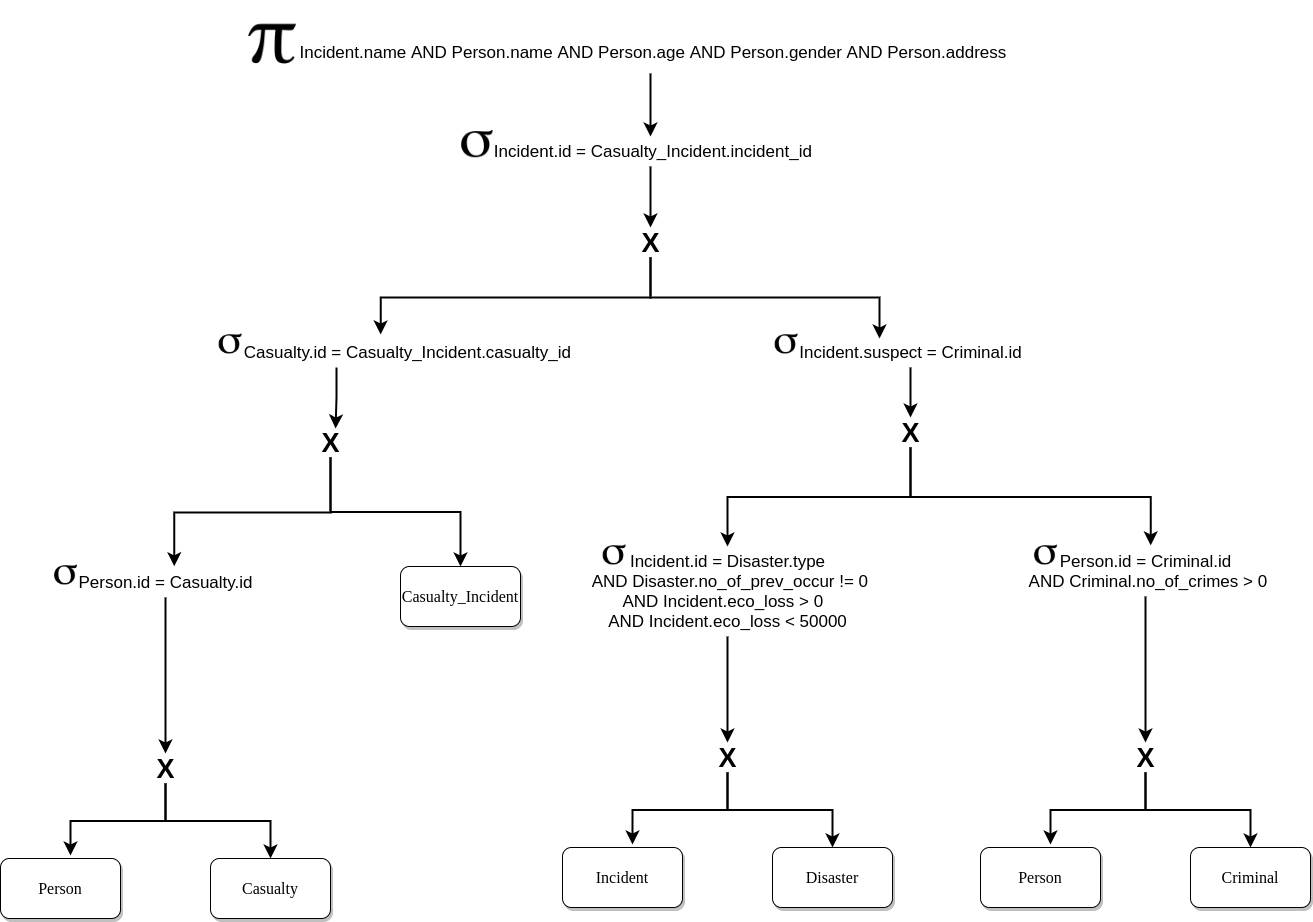
\includegraphics[width=0.8\textwidth]{images/query_trees/query5-non-optimized.png}
    \caption{Query tree for non-optimized query 5}
\end{figure}
\begin{figure}[H]
    \centering
    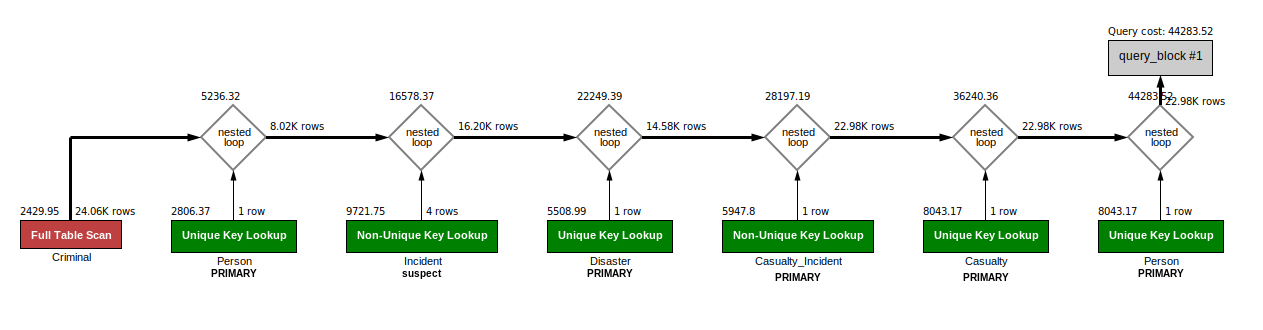
\includegraphics[width=\textwidth]{images/execution_plans/q5-1-old.png}
    \caption{Visual execution plan for non-optimized query 5}
\end{figure}

\subsubsection{Execution Plan After Optimization}
\begin{figure}[H]
    \centering
    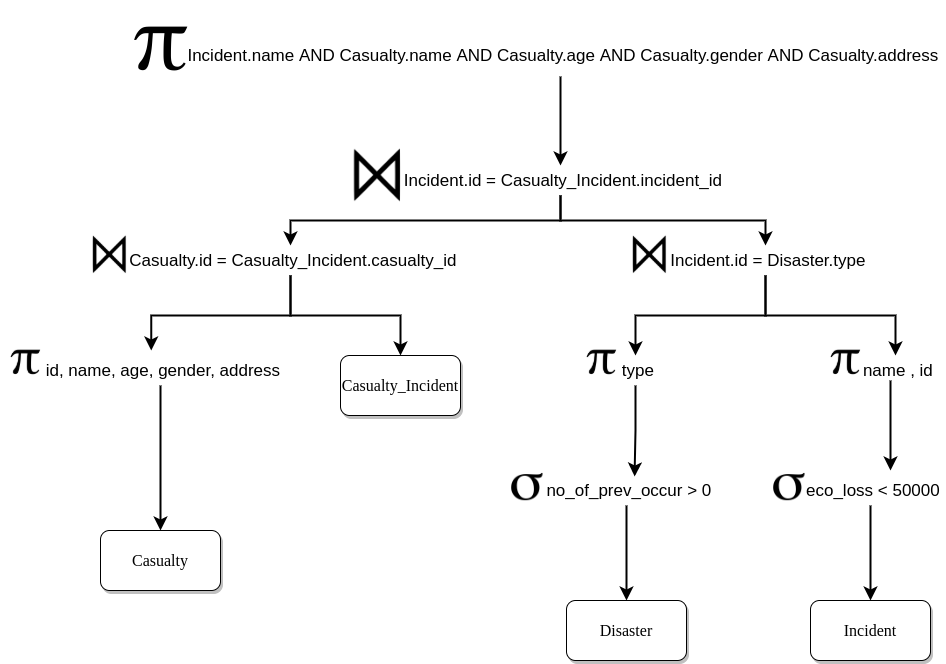
\includegraphics[width=0.8\textwidth]{images/query_trees/query5-optimized.png}
    \caption{Query tree for optimized query 5}
\end{figure}
\begin{figure}[H]
    \centering
    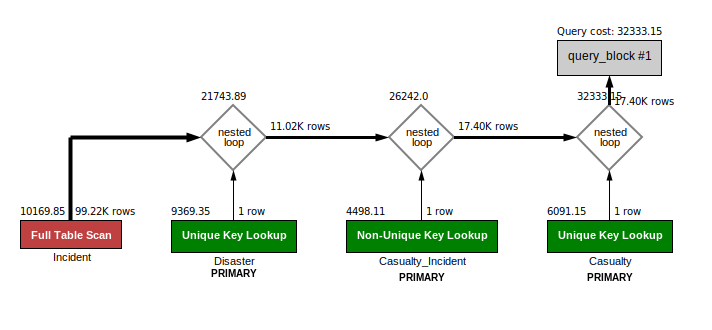
\includegraphics[width=\textwidth]{images/execution_plans/q5-4-new.png}
    \caption{Visual execution plan for optimized query 5}
\end{figure}
